\section{Theorie}
\label{sec:Theorie}

\subsection{Das Geiger-Müller-Zählrohr (GMZ)}

\begin{figure}
\centering
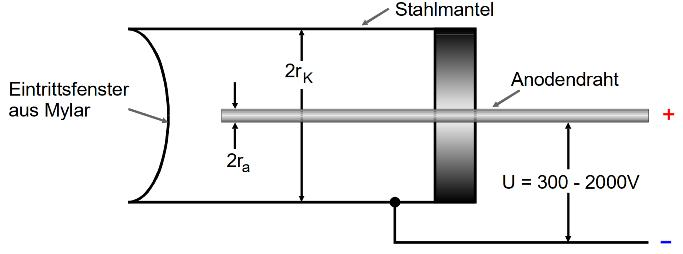
\includegraphics[scale=0.5]{content/images/aufbau1.jpg}
\caption{Aufbau eines Geiger-Müller-Zählrohrs \cite{V703}.}
\label{fig:GMZ}
\end{figure}
\noindent Das verwendete Zählrohr besteht, wie in Abbildung \ref{fig:GMZ} zu sehen ist, aus einem Zylindermantel aus Stahl, der als Kathode dient und einem Anodendraht. Zwischen Mantel und Draht wird eine Spannung von $U= 300 - 2000 \text{V}$ angelegt. Das dadurch entstehende elektrische Feld in Abhängigkeit vom Abstand $r$ zur Zählrohrachse ist gegeben durch
\[
E(r)=\frac{U}{r\ln\left(\frac{r_.K}{r_.A}\right)},
\]
wobei $r_.K$ und $r_.A$ die Radien des Zählrohrmantels bzw. des Drahtes sind.
Die eine Seite des Zylinders ist geschlossen auf der anderen befindet sich ein aus Mylarfolie bestehendes Endfenster, durch das die Teilchen eindringen können. Das Zählrohrinnere ist mit einem Argon-Gasgemisch gefüllt.
Dringen Teilchen durch das Fenster ein, wechselwirken sie mit dem Gas bis ihre gesamte Energie durch Ionisation und Anregung des Gases aufgebraucht ist.\newline
Abhängig von der angelegten Spannung (siehe Abbildung \ref{fig:AU})
kommen mehr oder weniger der ausgelösten Elektronen beim Draht an.
Bei niedrigen Spannungen Rekomibinieren viele der freien Elektronen schnell wieder mit den entstandenen Gasionen und gelangen somit nicht zum Draht (Bereich $I$, Abb.\ref{fig:AU}). Bei höheren Spannungen hingegen können die Elektronen so sehr beschleunigt werden, dass sie ihrerseits wieder durch Stöße das Gas weiter ionisieren und somit ihre Anzahl in einer Townsend-Lawine stark erhöhen \cite{V703} (Bereich $III$, Abb.\ref{fig:AU}).\newline
Bei weiterer Spannungserhöhung kommt es durch die vielen angeregten Gas-Atome zu Photonenemissionen, wenn diese in ihren Grundzustand zurückkehren. Da die Photonen neutral geladen sind, breiten sie sich auch senkrecht zum E-Feld aus, sodass sich die Elektronen-Lawine auf das ganze Zählrohr ausweitet. Dies ist der Geiger-Müller-Bereich, der als reiner Impulszähler dient (Bereich $IV$, Abb.\ref{fig:AU}).

\begin{figure}
\centering
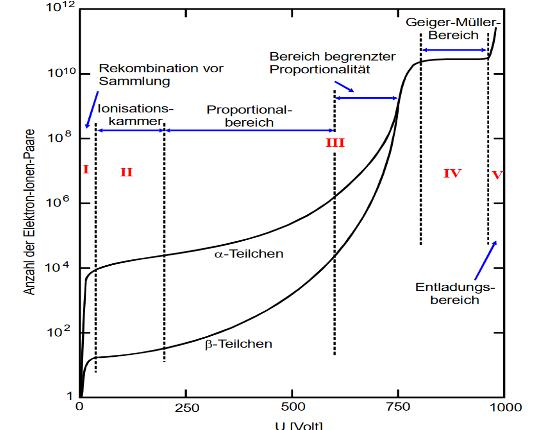
\includegraphics[scale=0.5]{content/images/AU.jpg}
\caption{Halblogarithmische Darstellung Elektronen-Ionen-Paare in Abhängigkeit von der Spannung $U$ \cite{V703}.}
\label{fig:AU}
\end{figure}

\subsection{Totzeit eines Geiger-Müller-Zählrohres}
Als Totzeit $T$ wird der Zeitraum bezeichnet, indem das Zählrohr unempfindlich gegen neue Anregungen durch eindringende Teilchen ist (siehe Abb.\ref{fig:TZ}).
Da sich die erzeugten Ionen auf Grund ihrer Trägheit für längere Zeit um den Anodendraht herum aufhalten und so das elektrische Feld schwächen, werden keine neuen Teilchen registriert, bis die Ionen zum Zylindermantel abwandern \cite{V703}. Die ursprüngliche Impulsstärke wird erst wieder erreicht, sobald alle Ionen neutralisiert sind. Die Zeit bis die ursprüngliche Impulsstärke wieder erreicht ist, wird Erholungszeit genannt.

\begin{figure}
\centering
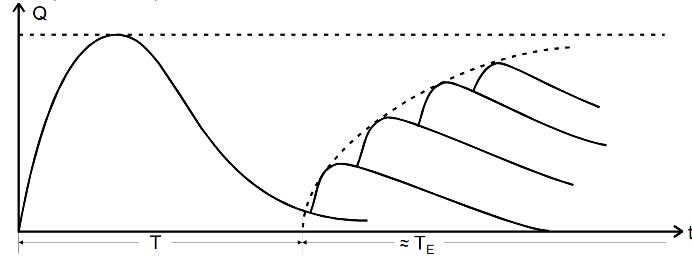
\includegraphics[scale=0.5]{content/images/T.jpg}
\caption{Ladung pro Teilchen in Abhängigkeit von der Zeit \cite{V703}.}
\label{fig:TZ}
\end{figure}

\subsubsection{Nachentladungen und Charakteristik des Geiger-Müller-Zählrohrs}
Bei der Neutralisation der Argon-Ionen entsteht bei ihrem Auftreffen auf den Zylindermantel genügend Energie, damit wieder Elektronen freigesetzt werden können, die auf ihrem Weg zum Anodendraht erneut Stoßionisationen ausführen und damit die Zählrohrentladung wieder neu zünden können.
So kann es ohne das ein neues Teilchen eingetreten ist zu mehreren zeitlich versetzten Impulsen kommen, wie sie in Abbildung \ref{fig:T} zu sehen sind. Zur Vermeidung solcher Nachentladungen können verschiedene Alkohol-Dämpfe zur Gasmischung hinzugefügt werden, die die Elektronen abfangen.\newline
Um die Qualität eines Zählrohrs zu bestimmen muss der Berreich $IV$ aus Abbildung \ref{fig:AU} genauer betrachtet werden. Die Abbildung \ref{fig:AU2} zeigt diesen Ausschnitt noch einmal vergrößert.
Der zu sehende lineare Teil des Graphen wird als Plateau bezeichnet und hätte bei einem idealen Zählrohr eine Steigung 0.
Es können jedoch nicht alle Nachentladungen durch Gaszusätze verhindert werden, sodass diese zu einem leichten Anstieg führen.
Je geringer dieser und je größer der Spannungsbereich des Plateaus, desto besser arbeitet das Zählrohr.

\begin{figure}
\centering
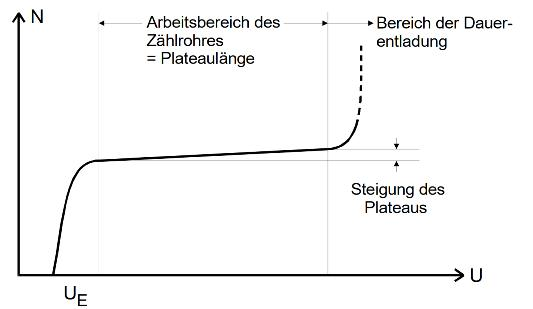
\includegraphics[scale=0.5]{content/images/AU2.jpg}
\caption{Charakteristik eines Geiger-Müller-Zählrohrs \cite{V703}.}
\label{fig:AU2}
\end{figure}

\subsubsection{Totzeit-Bestimmung: Zwei-Quellen-Methode}
Wegen der Totzeit $T$ kann das Geiger-Müller-Zählrohr nicht die wirkliche Impulsrate $N_.w$ messen, sondern nur eine Impulsrate $N_.r$ registrieren. Unter der vereinfachten Annahme, dass bei dieser Rate für den Teil $T\cdot N_.r$ der Zeit das Zählrohr unempfindlich ist, gilt:
\begin{equation}
N_.w=\frac{N_.r}{1-T\cdot N_.r}\label{eq:Zählrate}
\end{equation}
Wird $N_.1$ einer Probe gemessen und anschließend eine zweite Probe hinzugefügt und $N_.{1+2}$ gemessen, worauf die Zählrate $N_.2$ alleine gemessen wird, kann wegen der Totzeit beobachtet werden, dass 
\[
N_.{1+2} < N_.1 + N_.2
\]
gilt.
Da die wirklichen Zählraten aber unabhängig von $T$ sind folgt:
\[
N_.{w_.{1+2}} = N_.{w_.1} + N_.{w_.2}
\]
und mit \eqref{eq:Zählrate}
\[
\frac{N_.{1+2}}{1-T\cdot N_.{1+2}}=\frac{N_.1}{1-T\cdot N_.1}+\frac{N_.2}{1-T\cdot N_.2} \text{.}
\]
Mit der Annahme das $T^2N_.r^2<<1$ kann die Totzeit deshalb berechnet werden zu 
\begin{equation}
T=\frac{N_.1+N_.2-N_.{1+2}}{2N_.1N_.2}\label{eq:T}
\end{equation}
\subsection{Freigesetzte Ladungsmenge pro eindringendem Teilchen}
Für den im Zählrohr fließenden Strom gilt, wenn $Z$ Teilchen im Zeitraum $\Delta t$ eindringen:
\begin{equation}
I=\frac{\Delta Q}{\Delta t}\cdot Z \label{eq:I}\text{.}
\end{equation}
Da nur der zeitlich gemittelte Strom gemessen wird, gilt mit dem Ohmschen Gesetz:
\[
I=\frac{1}{\tau}\int_0^{\tau}\frac{U(t)}{R}\mathrm{d}t \text{.}
\]
Gleichsetzen liefert, das $\Delta Q$ abhängig von $U$ ist.